\documentclass[12pt,oneside]{article}

\usepackage{szablon_pokrywka}
% Jeśli szablon_pokrywka nie ładuje poniższych pakietów, dodaj je ręcznie:
% \usepackage{amsmath,amssymb}
% \usepackage{float}
% \usepackage{listings}
% \usepackage{booktabs}

\author{Mateusz Pokrywka, Maciej Pereślucha}
\studentID{177143, 177139}
\type{Dokumentacja projektu}
\course{Wizja komputerowa}
\title{Detekcja i klasyfikacja znaków drogowych}

\begin{document}

\maketitle
\tableofcontents
\clearpage

% =========================================================
\section{Opis problemu}
% =========================================================
Projekt dotyczy automatycznego wykrywania i rozpoznawania znaków drogowych na zdjęciach.
System najpierw lokalizuje znak na obrazie (detekcja), a następnie przypisuje go do jednej
z~predefiniowanych kategorii (klasyfikacja). Do obu zadań wykorzystano klasyczne metody
wizji komputerowej i klasyfikator SVM. Ze względu na realizację projektu w dwuosobowej
grupie, w porozumieniu z prowadzącą ograniczono zakres do 5 klas: STOP, ustąp
pierwszeństwa, zakaz wjazdu, droga z pierwszeństwem oraz ograniczenie prędkości do
30~km/h; zrezygnowano też z porównania z podejściami opartymi na głębokich sieciach
neuronowych (YOLOv8-nano).

% =========================================================
\section{Część teoretyczna}
% =========================================================
Poniżej opisano wszystkie metody i algorytmy użyte w projekcie -- od wstępnego
przetwarzania obrazu, przez ekstrakcję cech, aż po klasyfikację. Każdy etap uzupełniono
o konkretne parametry z implementacji.

% ---------------------------------------------------------
\subsection{Algorytmy i filtry przetwarzania obrazu}
% ---------------------------------------------------------

\subsubsection{Filtr Gaussa}
Filtr Gaussa rozmywa obraz, usuwając drobne szumy i zakłócenia. Matematycznie jest to
splot obrazu z dwuwymiarową funkcją Gaussa:
\begin{equation}
    G(x,\, y,\, \sigma) = \frac{1}{2\pi\sigma^2}
    \exp\!\left(-\frac{x^2 + y^2}{2\sigma^2}\right)
    \label{eq:gauss}
\end{equation}
Obraz wygładzony: $I_g(x,y) = I(x,y) * G(x,y,\sigma)$. W implementacji użyto jądra
$5 \times 5$ z automatycznym doborem $\sigma$ przez OpenCV
(\texttt{cv2.GaussianBlur(img, (5,5), 0)}). Rozmycie ogranicza ryzyko wykrycia
fałszywych krawędzi na późniejszym etapie HOG.

\subsubsection{Konwersja przestrzeni barw BGR\texorpdfstring{$\to$}{->}HSV
              i BGR\texorpdfstring{$\to$}{->}Grayscale}
Przestrzeń HSV rozdziela kolor (Hue -- odcień) od jasności (Value), co sprawia, że
progowanie kolorów działa stabilnie przy różnym oświetleniu. Kanały wyznaczane są ze
składowych RGB:
\begin{align}
    V &= \max(R,\,G,\,B) \label{eq:hsv_v}\\
    S &= \frac{V - \min(R,\,G,\,B)}{V} \label{eq:hsv_s}\\
    H &\in [0^\circ,\, 360^\circ) \quad\text{(wyznaczany z proporcji składowych RGB)}
    \label{eq:hsv_h}
\end{align}
W OpenCV kanał $H$ jest skalowany do $[0,\,180]$ (tj. $H_{cv} = H/2$), a $S$, $V \in
[0,\,255]$. Konwersja do skali szarości (potrzebna dla HOG) sprowadza obraz do jednego
kanału intensywności:
\begin{equation}
    I_{gray} = 0{,}114\,B + 0{,}587\,G + 0{,}299\,R
    \label{eq:gray}
\end{equation}

\subsubsection{Progowanie kolorów i maska binarna}
Piksel trafia do maski, jeśli jego wartości $(H_{cv}, S, V)$ mieszczą się w zadanym
przedziale. Czerwień jest specyficzna -- w przestrzeni HSV ``zawija się'' wokół
$0^\circ$, więc trzeba sprawdzać dwa osobne zakresy kątowe:
\begin{equation}
    H_{red} \in [0^\circ,\, 20^\circ) \;\cup\; [320^\circ,\, 360^\circ)
\end{equation}
W skali OpenCV ($H_{cv} = H/2$) odpowiada to następującym progom z kodu:
\begin{align}
    M_{red1}   &:\quad H_{cv}\!\in[0,10],\; S\!\in[30,255],\; V\!\in[40,255]
               \label{eq:red1}\\
    M_{red2}   &:\quad H_{cv}\!\in[160,180],\; S\!\in[30,255],\; V\!\in[40,255]
               \label{eq:red2}\\
    M_{yellow} &:\quad H_{cv}\!\in[20,35],\; S\!\in[100,255],\; V\!\in[100,255]
               \label{eq:yellow}
\end{align}
Wszystkie trzy maski łączone są w jedną maskę kombinowaną:
\begin{equation}
    M = M_{red1} \lor M_{red2} \lor M_{yellow}
    \label{eq:mask}
\end{equation}

\subsubsection{Morfologiczne filtry nieliniowe}
Operacje morfologiczne działają na czarno-białych maskach i pozwalają poprawić ich jakość
-- usunąć szum lub wypełnić dziury. Każda operacja korzysta z małego jądra $B$ (np.
$3\times3$ lub $7\times7$). Podstawowe operacje to erozja i dylatacja:
\begin{align}
    \text{Erozja:}\quad   (A \ominus B)(p) &= \min_{b \in B}\, A(p + b)
    \label{eq:erosion}\\
    \text{Dylatacja:}\quad (A \oplus B)(p)  &= \max_{b \in B}\, A(p + b)
    \label{eq:dilation}
\end{align}
Łącząc je, otrzymujemy dwie użyteczne operacje złożone:
\begin{align}
    \text{Otwarcie:}\quad  A \circ B   &= (A \ominus B) \oplus B
    \label{eq:opening}\\
    \text{Zamknięcie:}\quad A \bullet B &= (A \oplus B) \ominus B
    \label{eq:closing}
\end{align}
W implementacji stosowane są kolejno:
\begin{enumerate}
    \item otwarcie z jądrem $3 \times 3$ -- usuwa drobne szumy i pojedyncze piksele
          z tła maski,
    \item zamknięcie z jądrem $7 \times 7$ -- wypełnia dziury i luki wewnątrz
          wykrytych obiektów.
\end{enumerate}

\subsubsection{Detekcja konturów}
Na oczyszczonej masce szukamy konturów, czyli ciągłych obrysów obiektów, korzystając
z algorytmu Suzuki--Abe (\texttt{cv2.findContours}). Spośród wszystkich konturów
$\{C_i\}$ wybieramy ten o największej powierzchni -- zakładamy, że to nasz znak:
\begin{equation}
    C^* = \underset{C_i}{\arg\max}\; A(C_i)
    \label{eq:maxcontour}
\end{equation}

\subsubsection{Filtry geometryczne konturów}
Żeby odrzucić fałszywe detekcje (drzewa, budynki, pojazdy), każdy kandydat sprawdzany
jest pod kątem kształtu. Używamy dwóch prostych miar:
\begin{align}
    \text{aspect ratio} &= \frac{w}{h}
    \label{eq:ar}\\
    \text{solidity} &= \frac{A_{\text{contour}}}{A_{\text{convex hull}}} \;\in\; (0,\,1]
    \label{eq:solidity}
\end{align}
Znaki drogowe mają zbliżone proporcje ($\text{aspect ratio} \approx 1$) i wysoką
zwartość ($\text{solidity} \approx 1$), bo ich kształt (koło, trójkąt, ośmiokąt)
jest regularny. Obiekty odstające od tych wartości są odrzucane.

\subsubsection{Ekstrakcja ROI}
Po wybraniu konturu wycinamy z oryginalnego obrazu obszar zainteresowania (ROI --
Region of Interest). Dodajemy margines $m = \lfloor 0{,}05 \cdot b_w \rfloor$
(5\% szerokości), żeby nie obcinać krawędzi znaku:
\begin{equation}
    \text{ROI} = I[\,y_1:y_2,\; x_1:x_2\,], \qquad
    \begin{cases}
        x_1 = \max(0,\; b_x - m) \\
        y_1 = \max(0,\; b_y - m) \\
        x_2 = \min(W,\; b_x + b_w + m) \\
        y_2 = \min(H,\; b_y + b_h + m)
    \end{cases}
    \label{eq:roi}
\end{equation}
Jeśli segmentacja nie znajdzie żadnego konturu, ROI jest całym obrazem. Wycięty
fragment skalowany jest do $64 \times 64$ px przed dalszym przetwarzaniem.

% ---------------------------------------------------------
\subsection{Ekstrakcja cech -- deskryptor HOG}
% ---------------------------------------------------------
HOG \cite{dalal2005} (Histogram of Oriented Gradients) zamienia obraz na wektor liczb
opisujący rozkład krawędzi. To dobry deskryptor dla znaków, bo znaki różnią się
przede wszystkim kształtem, a HOG właśnie kształt koduje.

\subsubsection{Obliczanie gradientów}
Dla każdego piksela obrazu w skali szarości $I$ wyznaczamy pochodne kierunkowe
prostym operatorem różnicowym:
\begin{align}
    G_x(x,y) &= I(x+1,\,y) - I(x-1,\,y)\\
    G_y(x,y) &= I(x,\,y+1) - I(x,\,y-1)
\end{align}
Następnie obliczamy magnitudę i kierunek gradientu:
\begin{align}
    m(x,y)      &= \sqrt{G_x^2(x,y) + G_y^2(x,y)}
    \label{eq:magnitude}\\
    \theta(x,y) &= \arctan\!\left(\frac{G_y(x,y)}{G_x(x,y)}\right)
                   \bmod 180^\circ
    \label{eq:orientation}
\end{align}
Kierunek jest liczony w zakresie $[0^\circ, 180^\circ)$ -- bez znaku -- bo krawędź
pozioma wygląda tak samo z obu stron. To poprawia odporność na zmiany oświetlenia.

\subsubsection{Histogram orientacji w komórce}
Obraz dzielimy na siatkę małych komórek $p \times p$ pikseli (w implementacji
$p = 8$). Dla każdej komórki budujemy histogram $b = 9$ przedziałów orientacyjnych,
równomiernie pokrywających $[0^\circ,\,180^\circ)$ (co $20^\circ$ na przedział).
Wartość $k$-tego przedziału:
\begin{equation}
    h_k^{(c)} = \sum_{(x,y)\,\in\, c} m(x,y) \cdot \mathbf{1}\!\left[
        \theta(x,y) \in \left[\frac{180^\circ(k-1)}{b},\;
        \frac{180^\circ k}{b}\right)
    \right], \quad k=1,\ldots,b
    \label{eq:hogbin}
\end{equation}
Gradient o dużej magnitudzie ma większy wkład do histogramu niż słaby -- dlatego
używamy $m(x,y)$ jako wagi.

\subsubsection{Normalizacja bloków -- L2-Hys}
Żeby uniezależnić deskryptor od lokalnych zmian jasności, komórki grupujemy w bloki
$c \times c$ (w implementacji $c = 2$, czyli $2\times2$ komórki). Histogramy
wszystkich komórek bloku sklejamy w wektor $\mathbf{v} \in \mathbb{R}^{c^2 b}$
i normalizujemy metodą L2-Hys w trzech krokach:
\begin{align}
    \mathbf{v}'      &= \frac{\mathbf{v}}{\sqrt{\|\mathbf{v}\|_2^2 + \varepsilon^2}}
    \label{eq:l2norm}\\
    v''_i            &= \min\!\left(v'_i,\; 0{,}2\right) \qquad\text{(obcięcie)}
    \label{eq:clip}\\
    \mathbf{v}_{norm}&= \frac{\mathbf{v}''}{\sqrt{\|\mathbf{v}''\|_2^2 + \varepsilon^2}}
    \label{eq:renorm}
\end{align}
Obcięcie wartości powyżej $0{,}2$ (krok drugi) tłumi dominację silnych gradientów
np. od obwódki znaku, dzięki czemu wnętrze znaku ma większy wpływ na opis.

\subsubsection{Wymiar wektora cech}
Tabela~\ref{tab:hog_params} zestawia parametry HOG z implementacji.

\begin{table}[H]
\centering
\begin{tabular}{lcr}
    \toprule
    Parametr & Symbol & Wartość \\
    \midrule
    Rozmiar obrazu        & $W = H$ & 64 px \\
    Rozmiar komórki       & $p$     & 8 px  \\
    Komórek w bloku       & $c$     & 2     \\
    Przedziałów orientacji& $b$     & 9     \\
    \bottomrule
\end{tabular}
\caption{Parametry deskryptora HOG użyte w implementacji.}
\label{tab:hog_params}
\end{table}

Liczba bloków w każdym wymiarze (okno przesuwa się co 1 komórkę):
\begin{equation}
    n_{blocks} = \frac{W}{p} - c + 1 = \frac{64}{8} - 2 + 1 = 7
\end{equation}
Wymiar całego wektora cech:
\begin{equation}
    d_{HOG} = \underbrace{n_{blocks}^2}_{\text{liczba bloków}} \cdot
              \underbrace{c^2 \cdot b}_{\text{cech na blok}} =
              7^2 \cdot 2^2 \cdot 9 = 49 \cdot 36 = \mathbf{1764}
    \label{eq:hogdim}
\end{equation}
Każde zdjęcie w zbiorze uczącym reprezentowane jest jako wektor
$\mathbf{x} \in \mathbb{R}^{1764}$.

% ---------------------------------------------------------
\subsection{Klasyfikacja -- SVM}
% ---------------------------------------------------------

\subsubsection{Idea i sformułowanie optymalizacyjne}
SVM \cite{cortes1995} (Support Vector Machine) to klasyfikator, który szuka
hiperpłaszczyzny decyzyjnej $\mathbf{w}^T\mathbf{x} + b = 0$ maksymalnie oddzielającej
klasy od siebie (patrz Rys.~\ref{Fig:svm}). Im szerszy margines między klasami,
tym lepsza generalizacja na nowych danych. W wersji soft-margin, która dopuszcza
pewne błędy klasyfikacji, zadanie optymalizacji wygląda następująco:
\begin{equation}
    \min_{\mathbf{w},\, b,\, \boldsymbol{\xi}}\;
    \frac{1}{2}\|\mathbf{w}\|^2 + C\sum_{i=1}^{n}\xi_i
    \qquad\text{przy}\qquad
    y_i\!\left(\mathbf{w}^T\mathbf{x}_i + b\right) \geq 1 - \xi_i,\;\; \xi_i \geq 0
    \label{eq:svm_soft}
\end{equation}
Parametr $C$ steruje kompromisem -- duże $C$ oznacza, że błędy są mocno karane
(wąski margines, ryzyko overfittingu), małe $C$ pozwala na więcej błędów
treningowych w zamian za szerszy margines. W implementacji użyto jądra liniowego
(\texttt{kernel='linear'}) z domyślną wartością $C = 1{,}0$.

\begin{figure}[H]
\centering
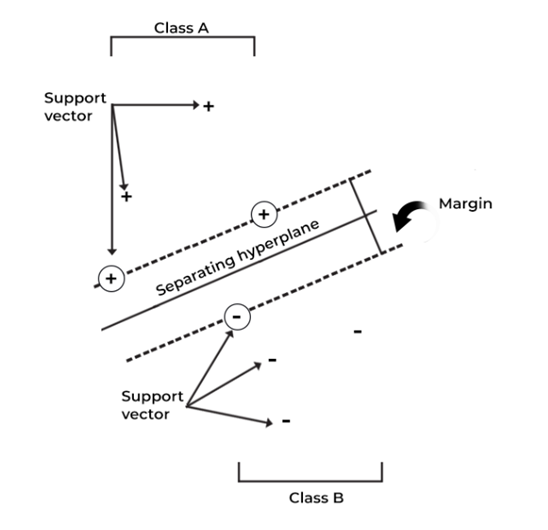
\includegraphics[width=14cm]{figures/obrazy/svm.png}
\caption{Hiperpłaszczyzna decyzyjna SVM z zaznaczonym marginesem i wektorami nośnymi.}
\label{Fig:svm}
\end{figure}

\subsubsection{Sformułowanie dualne i wektory nośne}
Równoważne, dualnie sformułowanie problemu pozwala wyrazić rozwiązanie przez punkty
treningowe przy użyciu mnożników Lagrange'a $\alpha_i \geq 0$:
\begin{equation}
    \max_{\boldsymbol{\alpha}}\;
    \sum_{i=1}^{n}\alpha_i - \frac{1}{2}\sum_{i,j=1}^{n}
    \alpha_i \alpha_j y_i y_j\, \mathbf{x}_i^T\mathbf{x}_j
    \qquad\text{przy}\qquad
    0 \leq \alpha_i \leq C,\;\; \sum_{i=1}^{n}\alpha_i y_i = 0
    \label{eq:svm_dual}
\end{equation}
Punkty, dla których $\alpha_i > 0$ nazywamy wektorami nośnymi (support vectors) --
to one wyznaczają hiperpłaszczyznę, reszta punktów treningowych nie ma znaczenia.
Funkcja decyzyjna:
\begin{equation}
    f(\mathbf{x}) = \text{sign}\!\left(
        \sum_{i:\,\alpha_i > 0} \alpha_i y_i\, \mathbf{x}_i^T\mathbf{x} + b
    \right)
    \label{eq:svm_decision}
\end{equation}

\subsubsection{Klasyfikacja wieloklasowa i estymacja prawdopodobieństwa}
SVM w podstawowej wersji rozwiązuje problem dwuklasowy. Scikit-learn rozszerza go
na wiele klas strategią jeden-na-jeden (OvO -- One vs One): dla każdej pary klas
trenowany jest osobny klasyfikator. Dla $K = 5$ klas daje to:
\begin{equation}
    \binom{K}{2} = \binom{5}{2} = 10 \quad\text{klasyfikatorów binarnych}
    \label{eq:ovo}
\end{equation}
Wynikowa klasa wyłaniana jest głosowaniem -- wygrywa ta, która wygrała najwięcej
pojedynków. Flaga \texttt{probability=True} w kodzie włącza skalowanie Platta,
które zamienia surowe wyniki klasyfikatorów na prawdopodobieństwa:
\begin{equation}
    P(y = k \mid \mathbf{x}) = \frac{1}{1 + e^{\,A_k f_k(\mathbf{x}) + B_k}}
    \label{eq:platt}
\end{equation}
Parametry $A_k$ i $B_k$ dopasowywane są automatycznie. Wartości te widoczne są
w kodzie jako \texttt{confidence} -- procent pewności klasyfikatora.

\subsubsection{Podział danych i metryki ewaluacyjne}
Zbiór 8370 próbek dzielony jest losowo w proporcji 80/20
(\texttt{random\_state=42} gwarantuje powtarzalność):
\begin{equation}
    |\mathcal{D}_{train}| = 0{,}8 \cdot 8370 = 6696 \qquad
    |\mathcal{D}_{test}|  = 0{,}2 \cdot 8370 = 1674
    \label{eq:split}
\end{equation}
Do oceny modelu używamy czterech standardowych metryk, wyznaczanych osobno dla
każdej klasy $k$, gdzie $TP_k$, $FP_k$, $FN_k$ to odpowiednio: prawdziwie pozytywne,
fałszywie pozytywne i fałszywie negatywne predykcje dla klasy $k$:
\begin{align}
    \text{Accuracy}    &= \frac{\displaystyle\sum_k TP_k}{n}
    \label{eq:accuracy}\\[4pt]
    \text{Precision}_k &= \frac{TP_k}{TP_k + FP_k}
    \label{eq:precision}\\[4pt]
    \text{Recall}_k    &= \frac{TP_k}{TP_k + FN_k}
    \label{eq:recall}\\[4pt]
    F_{1,k}            &= 2\cdot\frac{\text{Precision}_k \cdot \text{Recall}_k}
                                      {\text{Precision}_k + \text{Recall}_k}
    \label{eq:f1}
\end{align}

% =========================================================
\section{Analiza danych}
% =========================================================

\subsection{Dane do wytrenowania modelu SVM}
Do treningu użyto zbioru GTSRB (German Traffic Sign Recognition Benchmark)
\cite{stallkamp2012} -- jednego z najpopularniejszych zbiorów do rozpoznawania
znaków drogowych, zawierającego ponad 50\,000 zdjęć w 43 klasach. Korzystaliśmy
wyłącznie z części treningowej, ponieważ zdjęcia są tam posortowane według klas
i mają dostępne etykiety. Obrazy mają różne wymiary i zapisane są w formacie PNG
-- przeważającą część kadru zajmuje sam znak (patrz Rys.~\ref{Fig:przyk20kmh}).

\begin{figure}[H]
    \centering
    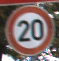
\includegraphics[width=14cm]{figures/obrazy/00000_00001_00029.png}
    \caption{Przykładowe zdjęcie z bazy GTSRB (klasa 0 --
             ograniczenie prędkości do 20 km/h).}
    \label{Fig:przyk20kmh}
\end{figure}

Spośród 43 klas wybraliśmy 5 odpowiadających zakresowi projektu:

\begin{table}[H]
\centering
\begin{tabular}{lc}
    \toprule
    Klasa & Liczba zdjęć \\
    \midrule
    Ograniczenie prędkości 30 km/h & 2220 \\
    Droga z pierwszeństwem         & 2100 \\
    Ustąp pierwszeństwa            & 2160 \\
    Zakaz wjazdu                   & 1110 \\
    STOP                           &  780 \\
    \midrule
    \textbf{Łącznie}               & \textbf{8370} \\
    \bottomrule
\end{tabular}
\caption{Liczebność poszczególnych klas w zbiorze uczącym.}
\label{tab:classes}
\end{table}

Zbiór podzielono losowo na treningowy (80\%) i testowy (20\%) funkcją
\texttt{train\_test\_split()} z biblioteki scikit-learn \cite{scikit}
(\texttt{random\_state=42} -- por. równanie~\ref{eq:split}).

\subsection{Dane do testowania procesu detekcji i klasyfikacji}
Do oceny całego potoku (nie tylko modelu SVM) użyliśmy zdjęć z polskich i~niemieckich
dróg pobranych z internetu. W odróżnieniu od GTSRB, zdjęcia te nie są posortowane
według klas, a znaki drogowe zajmują mniejszą część kadru -- bardziej zbliżone są do
warunków rzeczywistych (Rys.~\ref{Fig:znaki_testowe}).

\begin{figure}[H]
    \centering
    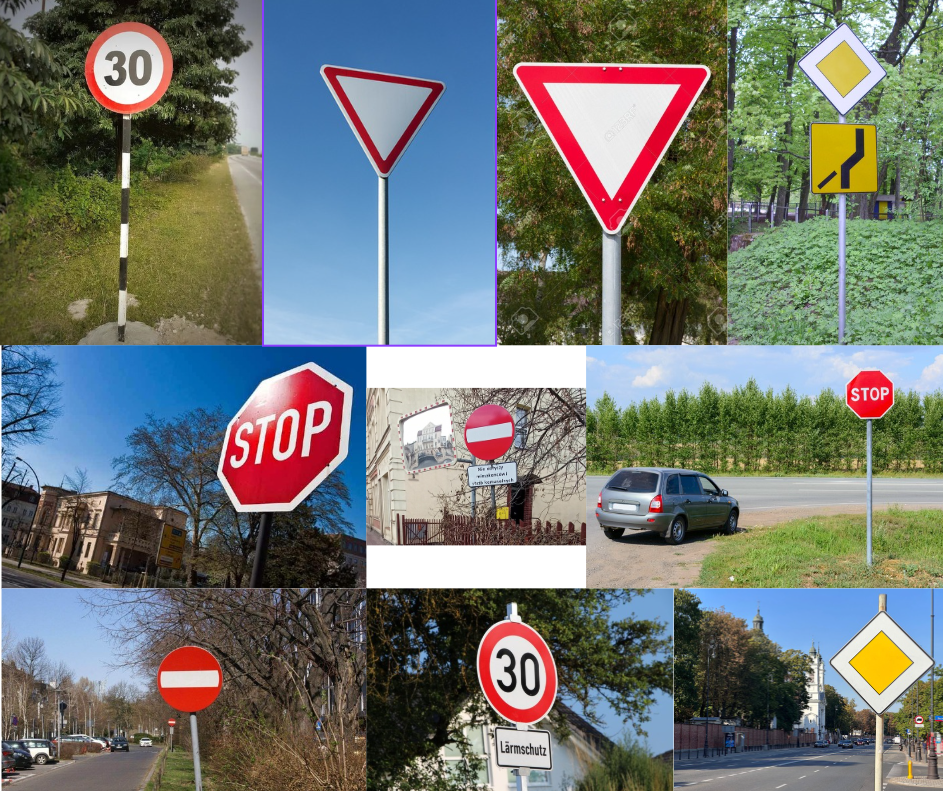
\includegraphics[width=14cm]{figures/obrazy/kolarz.png}
    \caption{Zestaw 10 zdjęć testowych do oceny skuteczności systemu.}
    \label{Fig:znaki_testowe}
\end{figure}

% =========================================================
\section{Pipeline procesu}
% =========================================================
Cały proces realizowany jest jako sekwencja pięciu etapów -- każdy etap przetwarza
wynik poprzedniego:

\begin{enumerate}

    \item \textbf{Wstępne przetwarzanie}: wczytanie obrazu, zastosowanie filtru Gaussa
    $5 \times 5$ (równanie~\ref{eq:gauss}), konwersja BGR$\to$HSV.

    \item \textbf{Segmentacja i binaryzacja}: progowanie trzech zakresów kolorów
    (równania \ref{eq:red1}--\ref{eq:yellow}) i połączenie masek
    (równanie~\ref{eq:mask}); następnie otwarcie jądrem $3\times3$ i zamknięcie
    jądrem $7\times7$ (równania \ref{eq:opening}--\ref{eq:closing}).

    \item \textbf{Detekcja i filtracja geometryczna}: wyznaczenie konturów,
    wybór największego (równanie~\ref{eq:maxcontour}), weryfikacja aspect ratio
    i solidity (równania \ref{eq:ar}--\ref{eq:solidity}).

    \item \textbf{Ekstrakcja ROI i cech}: wycięcie obszaru zainteresowania z marginesem
    5\% (równanie~\ref{eq:roi}), skalowanie do $64 \times 64$ px, konwersja do
    skali szarości, ekstrakcja wektora HOG $\in \mathbb{R}^{1764}$
    (równanie~\ref{eq:hogdim}).

    \item \textbf{Klasyfikacja SVM}: przekazanie wektora cech do wytrenowanego
    klasyfikatora liniowego SVM (równanie~\ref{eq:svm_decision}), przypisanie
    do jednej z 5 klas wraz z prawdopodobieństwem (równanie~\ref{eq:platt}).

\end{enumerate}

% =========================================================
\section{Skrypt programu}
% =========================================================

\begin{lstlisting}[language=Python,
    caption={Pełny potok treningu: preprocessing HSV + ekstrakcja HOG + SVM},
    label={lst:train}]
import os
import cv2
import numpy as np
from skimage.feature import hog
from sklearn.model_selection import train_test_split
from sklearn.svm import SVC
from sklearn.metrics import (accuracy_score, classification_report,
                             confusion_matrix, ConfusionMatrixDisplay)
import matplotlib.pyplot as plt
import joblib

DATA_DIR        = '../data/selected_signs'
MODEL_SAVE_PATH = '../models/svm_model.pkl'
IMG_SIZE        = (64, 64)

X, labels, rois_for_display = [], [], []
os.makedirs(os.path.dirname(MODEL_SAVE_PATH), exist_ok=True)

for class_name in os.listdir(DATA_DIR):
    class_path = os.path.join(DATA_DIR, class_name)
    if not os.path.isdir(class_path):
        continue
    for img_name in os.listdir(class_path):
        img_path = os.path.join(class_path, img_name)
        img = cv2.imread(img_path)
        if img is None or img.size == 0:
            print(f"[POMINIETO] Uszkodzony plik: {img_path}")
            continue
        try:
            # --- Etap 1: Odszumianie i maskowanie HSV ---
            img_blurred = cv2.GaussianBlur(img, (5, 5), 0)
            hsv = cv2.cvtColor(img_blurred, cv2.COLOR_BGR2HSV)

            # Czerwien w HSV dzieli sie na dwa zakresy katowe
            lower_red1,   upper_red1   = np.array([0,30,40]),   np.array([10,255,255])
            lower_red2,   upper_red2   = np.array([160,30,40]), np.array([180,255,255])
            lower_yellow, upper_yellow = np.array([20,100,100]),np.array([35,255,255])

            mask = (cv2.inRange(hsv, lower_red1,   upper_red1)   +
                    cv2.inRange(hsv, lower_red2,   upper_red2)   +
                    cv2.inRange(hsv, lower_yellow, upper_yellow))

            # OPEN 3x3 usuwa szum, CLOSE 7x7 wypelnia dziury w masce
            kernel_open  = np.ones((3, 3), np.uint8)
            kernel_close = np.ones((7, 7), np.uint8)
            mask = cv2.morphologyEx(mask, cv2.MORPH_OPEN,  kernel_open)
            mask = cv2.morphologyEx(mask, cv2.MORPH_CLOSE, kernel_close)

            contours, _ = cv2.findContours(
                mask, cv2.RETR_EXTERNAL, cv2.CHAIN_APPROX_SIMPLE)

            if contours:
                largest = max(contours, key=cv2.contourArea)
                bx, by, bw, bh = cv2.boundingRect(largest)
                margin = int(0.05 * bw)
                x1 = max(0, bx - margin)
                y1 = max(0, by - margin)
                x2 = min(img.shape[1], bx + bw + margin)
                y2 = min(img.shape[0], by + bh + margin)
                roi = img[y1:y2, x1:x2]
                if roi.size == 0:
                    roi = img.copy()
            else:
                roi = img.copy()

            # --- Etap 2: Resize -> Grayscale -> HOG ---
            # Parametry HOG daja wektor 1764 cech (patrz dokumentacja)
            img_resized = cv2.resize(roi, IMG_SIZE)
            gray = cv2.cvtColor(img_resized, cv2.COLOR_BGR2GRAY)
            features = hog(gray, orientations=9, pixels_per_cell=(8, 8),
                           cells_per_block=(2, 2), block_norm='L2-Hys',
                           visualize=False)

            X.append(features)
            labels.append(class_name)
            rois_for_display.append(cv2.cvtColor(roi, cv2.COLOR_BGR2RGB))

        except Exception as e:
            print(f"[BLAD] {img_path}: {e}")
            continue

X                = np.array(X)
y                = np.array(labels)
rois_for_display = np.array(rois_for_display, dtype=object)

print(f"[INFO] Przetworzono {len(X)} zdj. z {len(np.unique(y))} klas.")

# --- Trening ---
X_train, X_test, y_train, y_test, rois_train, rois_test = train_test_split(
    X, y, rois_for_display, test_size=0.2, random_state=42)

svm_model = SVC(kernel='linear', probability=True)
svm_model.fit(X_train, y_train)

# --- Ewaluacja ---
y_pred   = svm_model.predict(X_test)
accuracy = accuracy_score(y_test, y_pred)
print(f"\n[WYNIK] Accuracy: {accuracy * 100:.2f}%\n")
print(classification_report(y_test, y_pred))

# --- Zapis ---
joblib.dump(svm_model, MODEL_SAVE_PATH)
print(f"[SUKCES] Model zapisany: {MODEL_SAVE_PATH}")

# --- Wizualizacja 1: Macierz pomylek ---
cm   = confusion_matrix(y_test, y_pred, labels=svm_model.classes_)
disp = ConfusionMatrixDisplay(confusion_matrix=cm,
                               display_labels=svm_model.classes_)
fig, ax = plt.subplots(figsize=(10, 8))
disp.plot(cmap='Blues', ax=ax, xticks_rotation=45, values_format='d')
plt.title('Macierz Pomylek -- SVM (HOG + OpenCV)', fontsize=15,
          fontweight='bold')
plt.tight_layout()
plt.show()

# --- Wizualizacja 2: Galeria predykcji (po 1 przykladzie z klasy) ---
unique_classes = np.unique(y_test)
num_classes    = len(unique_classes)
fig2, axes2    = plt.subplots(1, num_classes, figsize=(18, 4))
fig2.suptitle('Predykcje na zbiorze testowym', fontsize=16,
              fontweight='bold', y=1.1)

if num_classes == 1:    # axes2 nie jest iterowalny dla 1 klasy
    axes2 = [axes2]

for i, cls in enumerate(unique_classes):
    idx            = np.where(y_test == cls)[0][0]
    feature_vector = X_test[idx].reshape(1, -1)
    true_label     = y_test[idx]
    display_img    = rois_test[idx]

    prediction = svm_model.predict(feature_vector)[0]
    confidence = np.max(svm_model.predict_proba(feature_vector)) * 100

    title_color = 'green' if prediction == true_label else 'red'
    axes2[i].imshow(display_img)
    axes2[i].set_title(
        f"Predykcja: {prediction}\nPewnosc: {confidence:.1f}%\n"
        f"Prawda: {true_label}",
        fontsize=11, color=title_color, fontweight='bold')
    axes2[i].axis('off')

plt.tight_layout()
plt.show()
\end{lstlisting}

% =========================================================
\section{Eksperymenty}
% =========================================================
Eksperymenty...

% =========================================================
\section{Podsumowanie i wnioski}
% =========================================================
Podsumowanie i wnioski...

% =========================================================
\begin{thebibliography}{9}

    \bibitem{dalal2005}
        N. Dalal, B. Triggs:
        \textit{Histograms of Oriented Gradients for Human Detection},
        CVPR 2005, San Diego, CA, s.~886--893.

    \bibitem{cortes1995}
        C. Cortes, V. Vapnik:
        \textit{Support-Vector Networks},
        Machine Learning, vol.~20, no.~3, 1995, s.~273--297.

    \bibitem{stallkamp2012}
        J. Stallkamp, M. Schlipsing, J. Salmen, C. Igel:
        \textit{Man vs. computer: Benchmarking machine learning algorithms
        for traffic sign recognition},
        Neural Networks, vol.~32, 2012, s.~323--332.

    \bibitem{scikit}
        F. Pedregosa et al.:
        \textit{Scikit-learn: Machine Learning in Python},
        JMLR, vol.~12, 2011, s.~2825--2830.

    \bibitem{opencv}
        G. Bradski:
        \textit{The OpenCV Library},
        Dr. Dobb's Journal of Software Tools, 2000.

\end{thebibliography}

\end{document}